\documentclass{beamer}

\usetheme{metropolis}           % Use metropolis theme
\title{Automatic Pattern Recognition in Solids
based on Machine Learning}
\subtitle{Project thesis Computational Physics}
\date{\today}
\author{Matthias Vogler}
\institute{Departement of Physics\\ University of Basel}

\usepackage[backend=biber,style=ieee,natbib=true]{biblatex} % Use the bibtex backend with the authoryear citation style (which resembles APA)

\addbibresource{example.bib} % The filename of the bibliography

\usepackage[autostyle=true]{csquotes} % Required to generate language-dependent quotes in the bibliography


\begin{document}
  \maketitle
\begin{frame}
  \frametitle{What was the task?}
  Using the fingerprint proposed by \citeauthor{Zhu2016} \cite{Zhu2016} and the maximum volume simplex method proposed by \citeauthor{Behnam2020} \cite{Behnam2020} to classify constituent atoms in carbon-nitrate crystals
\end{frame}

\begin{frame}
  \frametitle{The data}
  I used the carbon-nitrate crystal structures provided by Prof. Alireza Ghasemi. For calculations used were
  \begin{itemize}
    \item 99 crystals with 8 atoms per cell
    \item 4949 crystals with 16 atoms per cell

  \end{itemize}

\end{frame}

\begin{frame}
\frametitle{What does the data look like?}
  \begin{figure}[h!]
    \center
    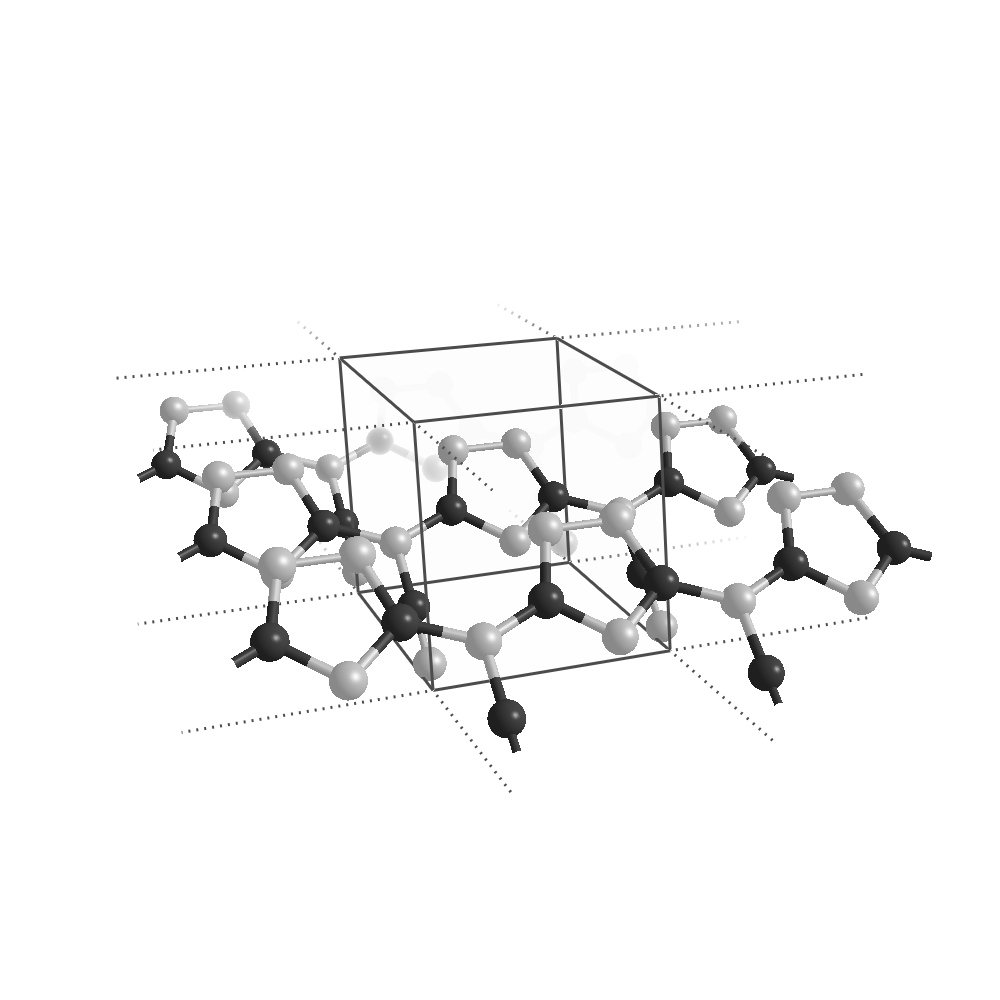
\includegraphics[scale=0.19]{Figures/8structure.png}
    \label{fig:8struct}
    \caption{Carbon-nitrate structre with 8 atoms per unit cell. White: Nitrogen, Black: Carbon}
  \end{figure}
\end{frame}



\begin{frame}
  \frametitle{The Procedure}
  The fingerprint algorithm was modified to include the 2s and 2p eigenenergies of carbon and nitrogen in the Gaussian type orbitals (GTO).
  \begin{itemize}
    \item Overlap integral (for s-s): $S_{ji}=\left(\frac{2\sqrt{\alpha_i\alpha_j}}{\alpha_i+\alpha_j}\right)^\frac{3}{2}\exp\left[\frac{-\alpha_i\alpha_j}{\alpha_i+\alpha_j}r_{ij}^2\right]$
    \item Gaussian width: $\tilde{\alpha}_i=C\cdot\frac{\alpha_i}{\left|E_{Orbital}\right|}$
    \item $C$ was empiricly determined to $C=0.19$
  \end{itemize}
\end{frame}


\begin{frame}
  \frametitle{The Procedure}
  \begin{table}[h!]
\center
\label{table:energies}
\begin{tabular}{c|c|c}
            & \textbf{C} & \textbf{N} \\ \hline
2s {[}eV{]} & -0.500866  & -0.676151  \\ \hline
2p {[}eV{]} & -0.199186  & -0.266297 
\end{tabular}
\caption{2s and 2p orbital eigenenergies of N and C.}
\end{table}

\end{frame}

\begin{frame}
  \frametitle{The Procedure}
  \begin{figure}[h!]
    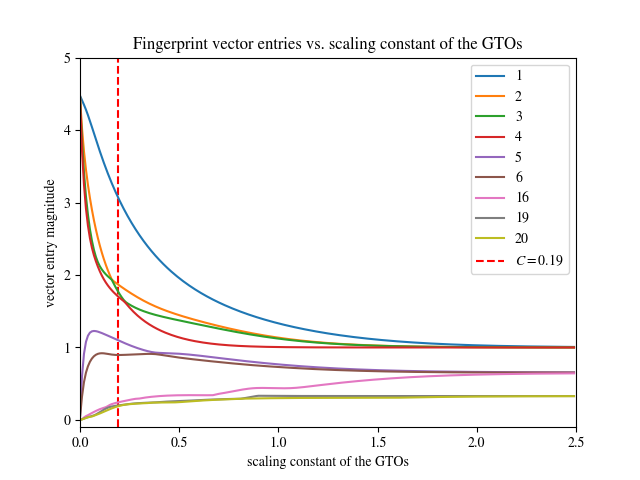
\includegraphics[scale=0.5]{Figures/fpentry.png}
    \caption{Plot of the fingerprint vector entries enumerated vs. the scaling constant $C$ of the GTO width.}
    \label{fig:const} 
  \end{figure}

\end{frame}

\begin{frame}
  \frametitle{The Procedure}
  \begin{enumerate}
    \item Calculate reference fingerprints out of reference structures
    \item Calculate maximum volume simplex out of the reference fingerprints
    \item Calculate validation fingerprints out of validation structures
    \item Search for closest corner of simplex to fingerprint vector and classify the atom
  \end{enumerate}
  Compiling and executing the different fortran scrpits was done with a simple bash script
\end{frame}

\begin{frame}
  \frametitle{Landmark structures: Examples}
    \begin{figure}[h!]
    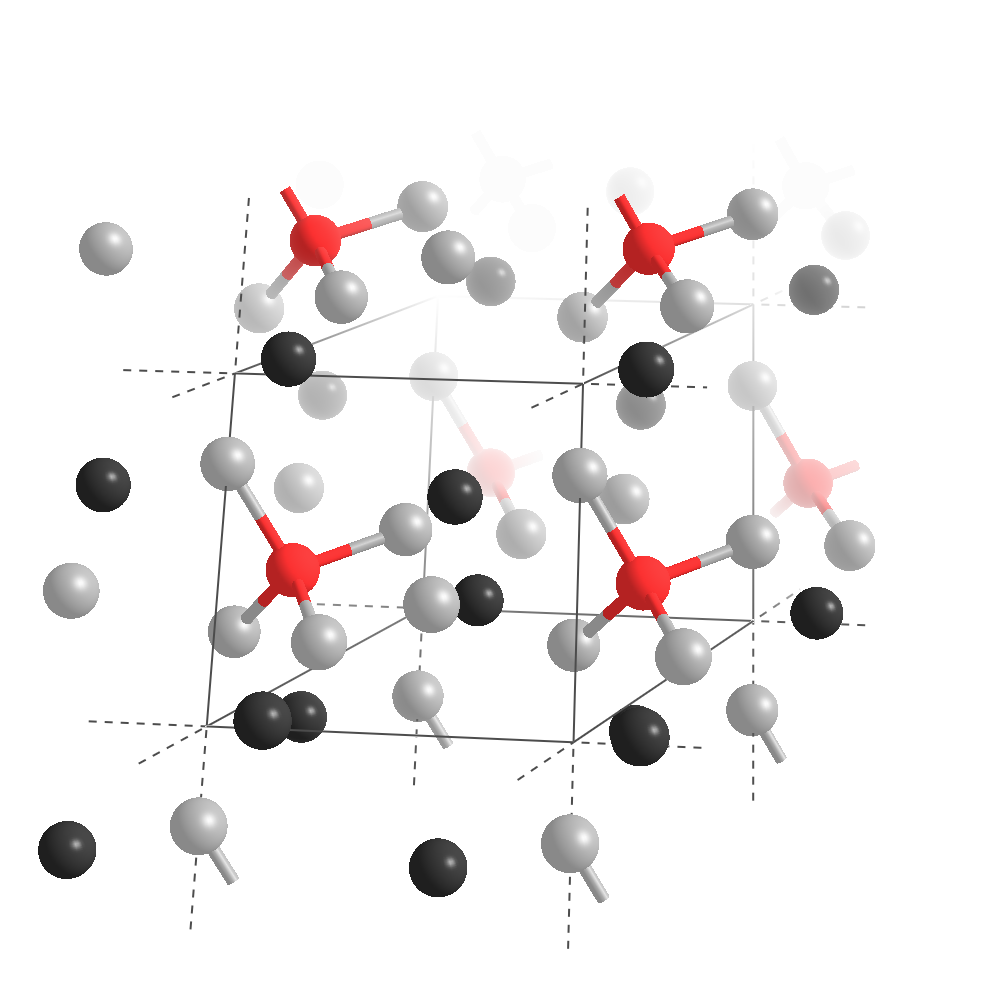
\includegraphics[scale=0.19]{Figures/landmark1.png}
    \caption{Four-coordinated carbon with 4 nitrogen neighbours; black: carbon; white: nitrogen; red: carbon center atom.}
    \label{fig:const} 
  \end{figure}
\end{frame}

\begin{frame}
  \frametitle{Landmark structures: Examples}
    \begin{figure}[h!]
    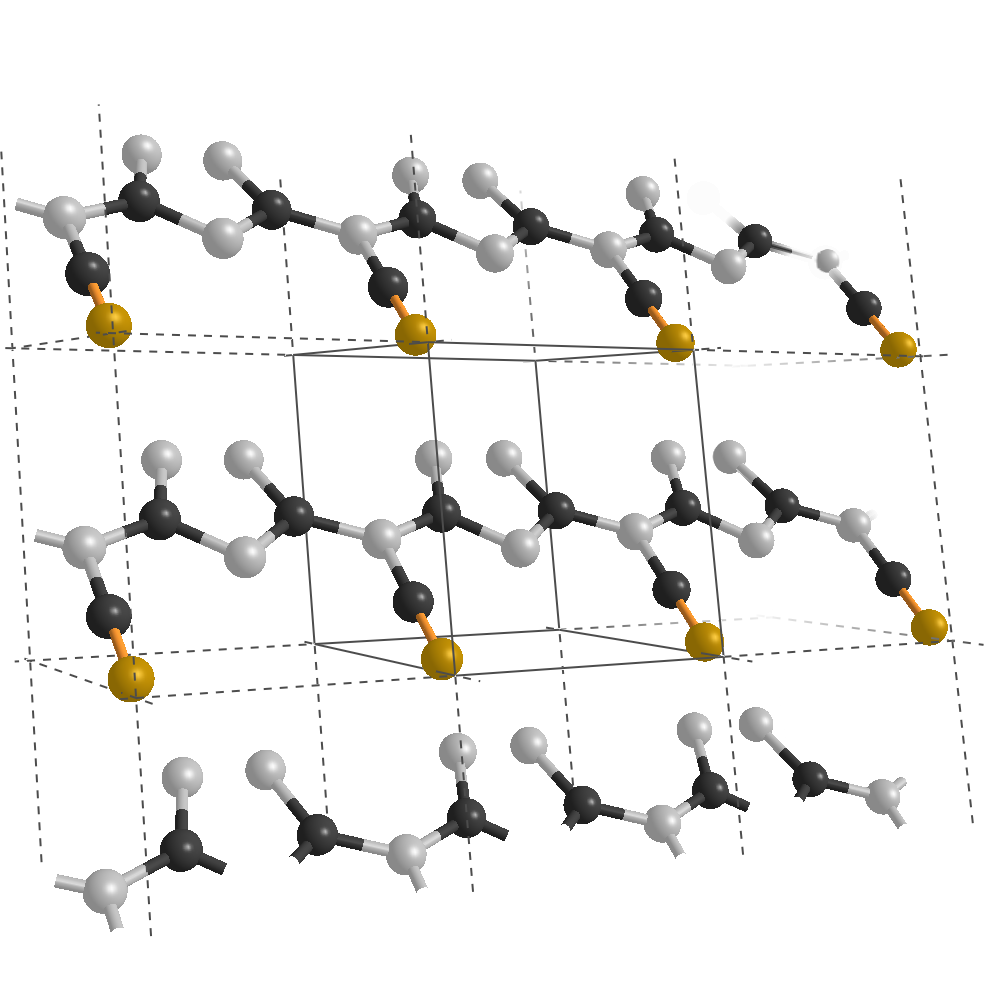
\includegraphics[scale=0.19]{Figures/landmark2.png}
    \caption{One-coordinated nitrogen}
    \label{fig:const} 
  \end{figure}
\end{frame}

\begin{frame}
  \frametitle{Landmark structures: Examples}
    \begin{figure}[h!]
    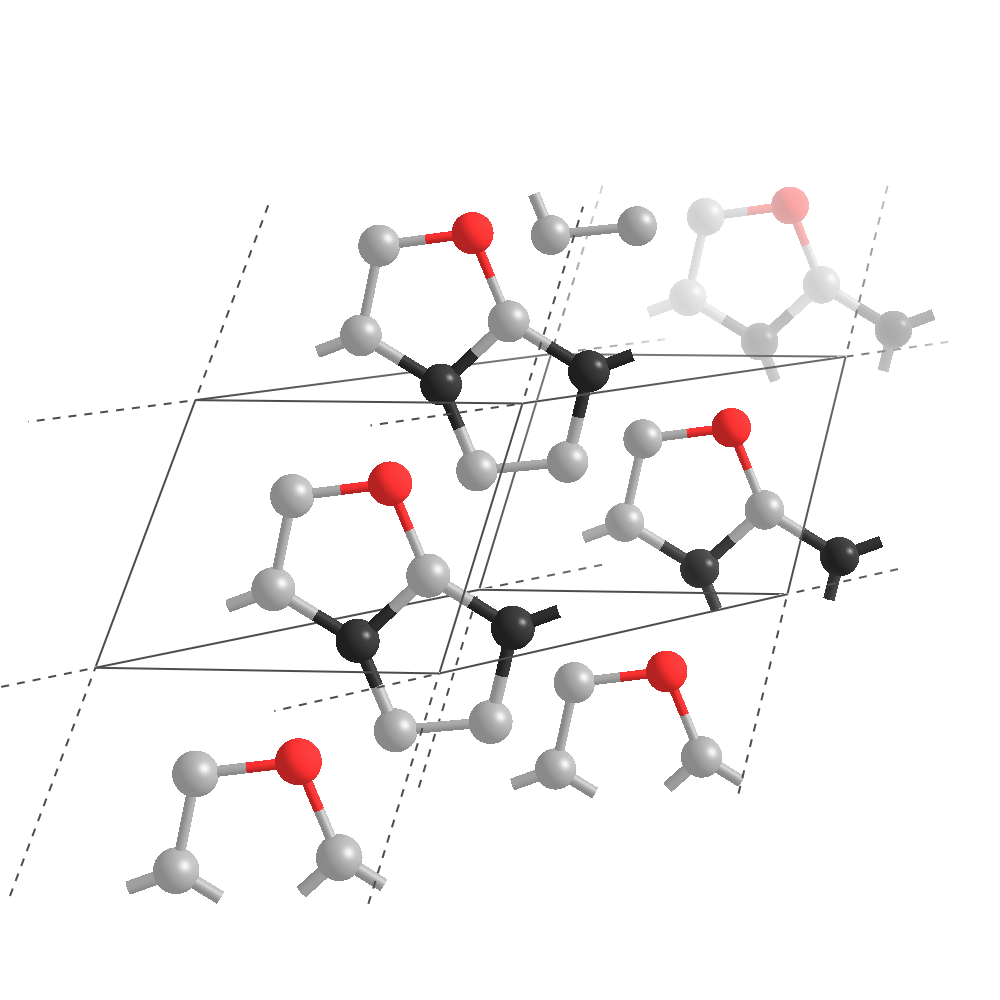
\includegraphics[scale=0.19]{Figures/landmark3.png}
    \caption{Two-coordinated carbon}
    \label{fig:const} 
  \end{figure}
\end{frame}

\begin{frame}
  \frametitle{Landmark structures: Examples}
    \begin{figure}[h!]
    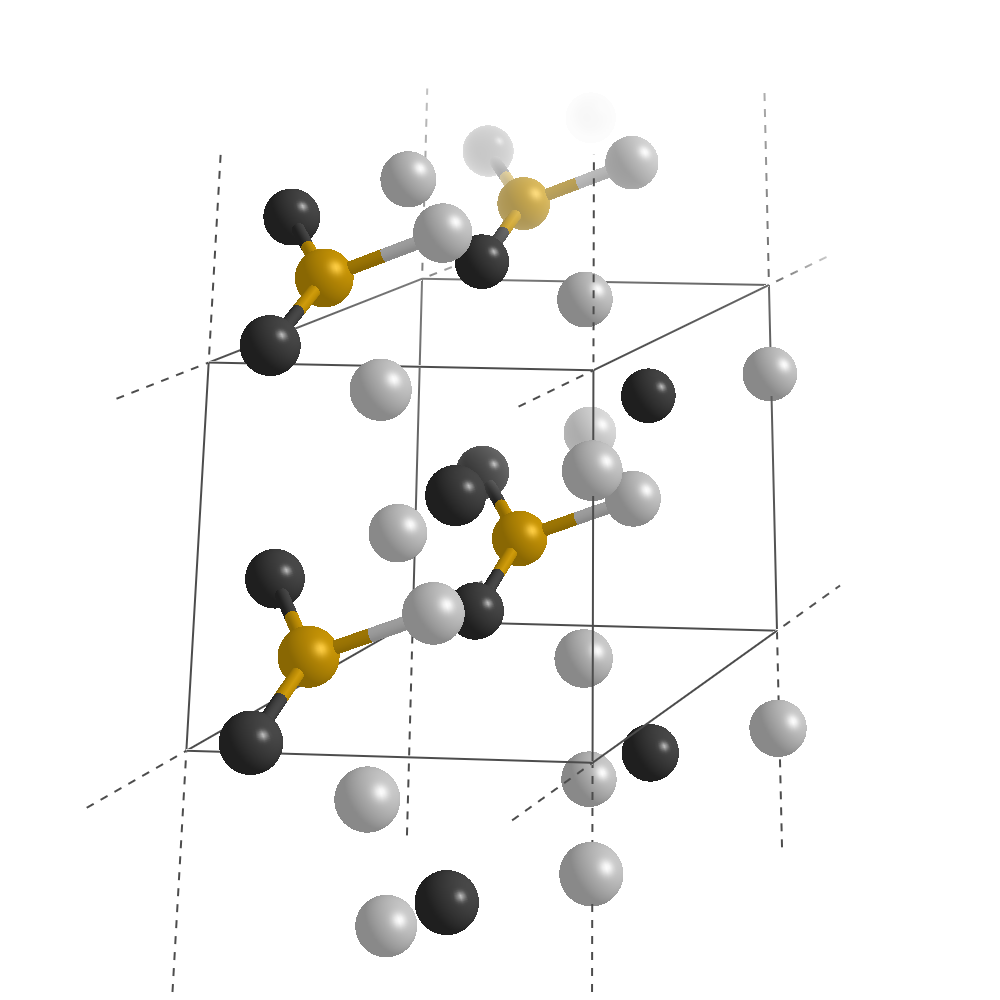
\includegraphics[scale=0.19]{Figures/landmark4.png}
    \caption{Three-coordinated nitrogen with 3 carbon and 1 nitrogen neighbour}
    \label{fig:const} 
  \end{figure}
\end{frame}

\begin{frame}
  \frametitle{Training on 8 atom crystals: Results}
  \begin{table}[h!]
    \center
    \begin{tabular}{c|c|c|c}
      classification & correct & false & correct (relative) \\ \hline
      C              & 26497   & 4064  & 0.867              \\ \hline
      N              & 45426   & 3197  & 0.934              \\ \hline
      Total          & 71923   & 7261  & 0.908             
    \end{tabular}
    \caption{Classification results for the 4949 carbon nitrate crystals with 16 atoms per cell (79184 atoms in total) trained on 99 crystals with 8 atoms per cell.}
    \label{table:res1}
  \end{table}
\end{frame}


\begin{frame}
  \frametitle{Training on 16 atom crystals: Results}
  \begin{table}[h!]
    \center
    \begin{tabular}{c|c|c|c}
      classification & correct & false & correct (relative) \\ \hline
      C              & 21151   & 3917  & 0.844              \\ \hline
      N              & 45573   & 8543  & 0.842              \\ \hline
      Total          & 66724   & 12460  & 0.843             
    \end{tabular}
    \caption{Classification results for the 4949 carbon nitrate crystals with 16 atoms per cell (79184 atoms in total) trained on 63 crystals with 16 atoms per cell.}
    \label{table:res2}
  \end{table}
\end{frame}

\begin{frame}
  \frametitle{Comparison to Supervised Learning: Random Forest}
  \begin{table}[h!]
\center
\begin{tabular}{c|c|c|c}
classification & correct & false & correct (relative) \\ \hline
C              & 8383   & 1475  & 0.850              \\ \hline
N              & 16128   & 407  & 0.975              \\ \hline
Total          & 24511   & 1881  & 0.929             
\end{tabular}
\caption{Classification results for $1/3$ of the 79184 environments (26395 in total) of the 16 atom structures averaged over 10 tries.}
\label{table:res3}
\end{table}
I used the implementation of the Random Forest Classifier implemented for Python in scikit-learn by \citeauthor{scikit} \cite{scikit}. 

\end{frame}

\begin{frame}
  \center
  \Huge
  Questions?

\end{frame}

































\begin{frame}
    \printbibliography[heading=bibintoc]

  \end{frame}
\end{document}